% Copyright (C) 2010,2012,2013 The ESPResSo project
% Copyright (C) 2002,2003,2004,2005,2006,2007,2008,2009,2010 
%   Max-Planck-Institute for Polymer Research, Theory Group
%  
% This file is part of ESPResSo.
%   
% ESPResSo is free software: you can redistribute it and/or modify it
% under the terms of the GNU General Public License as published by the
% Free Software Foundation, either version 3 of the License, or (at your
% option) any later version.
%  
% ESPResSo is distributed in the hope that it will be useful, but
% WITHOUT ANY WARRANTY; without even the implied warranty of
% MERCHANTABILITY or FITNESS FOR A PARTICULAR PURPOSE.  See the GNU
% General Public License for more details.
%  
% You should have received a copy of the GNU General Public License
% along with this program.  If not, see <http://www.gnu.org/licenses/>.
%
\chapter{The MMM family of algorithms}
\label{chap:mmm}

\section{Introduction}

\todo{Cleanup: References, mathematics} In the MMM family of
algorithms for the electrostatic interaction, a convergence factor
approach to tackle the conditionally convergent Coulomb sum is used
(even the authors of the original MMM method have no idea what this
acronym stands for). Instead of defining the summation order, one
multiplies each summand by a continuous factor
$c(\beta,r_{ij},n_{klm})$ such that the sum is absolutely convergent
for $\beta>0$, but $c(0,.,.)=1$. The energy is then defined as the
limit $\beta\rightarrow 0$ of the sum, i. e. $\beta$ is an artificial
convergence parameter. For a convergence factor of $e^{-\beta
  n_{klm}^2}$ the limit is the same as the spherical limit, and one
can derive the classical Ewald method quite conveniently through this
approach \citep{smith81a}. To derive the formulas for MMM, one has to
use a different convergence factor, namely
$e^{-\beta|r_{ij}+n_{klm}|}$, which defines the alternative energy

\[ \tilde{E}=\,\frac{1}{2}\lim_{\beta\rightarrow
  0}\sum_{k,l,m}{\sum_{i,j=1}^N}' \frac{q_i q_je^{-\beta|p_{ij} +
    n_{klm}|}} {|p_{ij} + n_{klm}|}
=:\,\frac{1}{2}\lim_{\beta\rightarrow 0}\sum_{i,j=1}^N
q_iq_j\phi_\beta(x_{ij}, y_{ij},z_{ij}). \]

$\phi_\beta$ is given by $ \phi_\beta(x,y,z)=\,\tilde\phi_\beta(x,y,z)
+ \frac{e^{-\beta r}}{r} $ for $(x,y,z)\neq 0$ and
$\phi_\beta(0,0,0)=\,\tilde\phi_\beta(0,0,0)$, where

\[ \tilde\phi_\beta(x,y,z)=\,\sum_{(k,l,m)\neq 0} \frac{e^{-\beta
    r_{klm}}}{r_{klm}}. \]

The limit $\tilde{E}$ exists, but differs for three dimensionally
periodic systems by some multiple of the square of the dipole moment
from the spherical limit as obtained by the Ewald
summation\citep{smith81a}. From the physical point of view the Coulomb
interaction is replaced by a screened Coulomb interaction with
screening length $1/\beta$. $\tilde{E}$ is then the energy in the
limit of infinite screening length. But because of the conditional
convergence of the electrostatic sum, this is not necessarily the same
as the energy of an unscreened system. Since the difference to the
Ewald methods only depends on the dipole moment of the system, the
correction can be calculated easily in linear time and can be ignored
with respect to accuracy as well as to computation time.

For one or two dimensionally systems, however, $\tilde{E}=E$, \ie the
convergence factor approach equals the spherical summation limit of
the Ewald sum, and MMM1D and MMM2D do not require a dipole correction.

Starting from this convergence factor approach, Strebel constructed a
method of computational order $O(N\log N)$, which is called MMM
\citep{strebel99a}. The favourable scaling is obtained, very much like
in the Ewald case, by technical tricks in the calculation of the far
formula.  The far formula has a product decomposition and can be
evaluated hierarchically similarly to the fast multipole methods.

For particles sufficiently separated in the z-axis one can Fourier
transform the potential along both x and y. We obtain the far formula
as

\[ \phi(x,y,z) =\, u_x u_y\sum_{p,q\neq 0} \frac{e^{2\pi f_{pq}z} +
  e^{2\pi f_{pq}(\lambda_z-z)}}{f_{pq} \left(e^{2\pi f_{pq}\lambda_z}
    - 1\right)} e^{2\pi i u_y q y}e^{2\pi i u_x p x} + 2\pi u_x
u_y\left(u_z z^2 - z + \frac{\lambda_z}{6}\right). \]

where $\lambda_{x,y,z}$ are the box dimensions, $ f_{pq} =\,
\sqrt{(u_x p)^2 + (u_y q)^2},\quad f_p =\, u_x p,\quad f_q =\, u_x q
$, $ \omega_p=2\pi u_x p$ and $\omega_q=2\pi u_y q$. The advantage of
this formula is that it allows for a product decomposition into
components of the particles. For example

\[ e^{2\pi f_{pq}z}=e^{2\pi f_{pq}(z_i-z_j)}=e^{2\pi
  f_{pq}z_i}e^{-2\pi f_{pq}z_j} \]

etc. Therefore one just has to calculate the sum over all these
exponentials on the left side and on the right side and multiply them
together, which can be done in $O(N)$ computation time. As can be seen
easily, the convergence of the series is excellent as long as z is
sufficiently large. By symmetry one can choose the coordinate with the
largest distance as z to optimise the convergence. Similar to the
Lekner sum, we need a different formula if all coordinates are small,
i. e. for particles close to each other. For sufficiently small
$u_y\rho$ and $u_xx$ we obtain the near formula as

\[ \begin{array}{rl} \tilde\phi(x,y,z)=\, & 2 u_x
  u_y\sum\limits_{p,q>0} \frac{\cosh(2\pi f_{pq}z)}{f_{pq}
    \left(e^{2\pi f_{pq}\lambda_z} - 1\right)} e^{2\pi i u_y q
    y}e^{2\pi i u_x p x} +\\ & 4u_x\sum\limits_{l,p>0}\left(K_0(2\pi
    u_x p\rho_l) + K_N(2\pi u_x p\rho_{-l})\right)cos(2\pi u_x p x)
  -\\ & 2u_x\sum\limits_{n\ge 1}\frac{b_{2n}}{2n(2n)!}\Re\bigl((2\pi
  u_y (z+iy))^{2n}\bigr) +\\ & u_x\sum\limits_{n\ge
    0}\left(\begin{array}{c}-\frac{1}{2}\\
      n\end{array}\right)\frac{\left( \psi^{(2n)}(1 + u_x x) +
      \psi^{(2n)}(1 - u_x x)\right)}{(2n)!}\rho^{2n} -\\ &
  2\log(4\pi). \end{array} \]

Note that this time we calculate $\tilde{\phi}$ instead of $\phi$, i.
e. we omit the contribution of the primary simulation box. This is
very convenient as it includes the case of self energy and makes
$\tilde{\phi}$ a smooth function. To obtain $\phi$ one has to add the
$1/r$ contribution of the primary box. The self energy is given by

\[ \tilde\phi(0,0,0)=\, 2 u_x u_y\sum\limits_{p,q>0} \frac{1}{f_{pq}
  \left(e^{2\pi f_{pq}\lambda_z} - 1\right)}+
8u_x\sum\limits_{l,p>0}K_N(2\pi u_x\lambda_y p l) + 2 u_x\psi^{(0)}(1)
- 2\log(4\pi). \]

Both the near and far formula are derived using the same convergence
factor approach, and consequently the same singularity in $\beta$ is
obtained. This is important since otherwise the charge neutrality
argument does not hold.

To obtain the $O(N\log N)$ scaling, some algorithm tricks are needed,
which are not used in MMM1D, MMM2D or ELC and are therefore not
discussed here. For details, see \citet{strebel99a}. MMM is not
implemented in \es.

\section{MMM2D}

In the case of periodicity only in the x and y directions, the far
formula looks like

\[ \begin{array}{rl} \phi(x,y,z) = \, & 4 u_x u_y\sum_{p,q>0}
  \frac{e^{-2\pi f_{pq}|z|}} {f_{pq}} \cos(\omega_p x)\cos(\omega_q y)
  +\\ & 2 u_x u_y\left(\sum_{q>0} \frac{e^{-2\pi f_q|z|}}{f_q}
    \cos(\omega_q y) + \sum_{p>0} \frac{e^{-2\pi f_p|z|}}{f_p}
    \cos(\omega_p x)\right) -\\ & 2\pi u_x u_y |z| \end{array} \],

and the near formula is

\[ \begin{array}{rl} \tilde\phi(x,y,z)=\, &
  4u_x\sum_{l,p>0}\left(K_0(\omega_p\rho_l) +
    K_0(\omega_p\rho_{-l})\right)\cos(\omega_p x) -\\ & 2u_x\sum_{n\ge
    1}\frac{b_{2n}}{2n(2n)!} \Re\bigl((2\pi u_y
  (z+iy))^{2n}\bigr)\,+\, \sum_{k=1}^{N_\psi-1}\left(\frac{1}{r_{k}} +
    \frac{1}{r_{-k}}\right) -\\ & u_x\sum_{n\ge
    0}\left(\begin{array}{c}-\frac{1}{2}\\n\end{array}\right)\frac{\left(
      \psi^{(2n)}(N_\psi + u_x x) + \psi^{(2n)}(N_\psi - u_x
      x)\right)}{(2n)!}(u_x\rho)^{2n} -\\ &
  2u_x\log\left(4\pi\frac{u_y}{u_x}\right). \end{array} \]

As said before, the energy obtained from these potentials is equal to
the electrostatic energy obtained by the spherical summation limit.
The deeper reason for this is that in some sense the electrostatic sum
is absolutely convergent \citep{mmm2d}.

The near formula is used for particles with a small distance along the
z axis, for all other particles the far formula is used. Below is
shown, that the far formula can be evaluated much more efficiently,
however, its convergence breaks down for small z distance. To
efficiently implement MMM2D, the layered cell system is required,
which splits up the system in equally sized gaps along the z axis. The
interaction of all particles in a layer S with all particles in the
layers S-1,S,S+1 is calculated using the near formula, for the
particles in layers $1,\dots,S-2$, and in layers $S+2,\dots,N$, the
far formula is used.

The implementation of the near formula is relatively straight forward
and can be treated as any short ranged force is treated using the link
cell algorithm, here in the layered variant. The special functions in
the formula are somewhat demanding, but for the polygamma functions
Taylor series can be achieved, which are implemented in mmm-common.h.
The Bessel functions are calculated using a Chebychev series.

The treatment of the far formula is algorithmically more complicated.
For a particle i in layer $ S_i$, the formula can product decomposed,
as in

\[ \begin{array}{rl} \sum_{j\in I_S, S < S_i - 1} q_iq_j\frac{e^{-2\pi
      f_{pq}|z_i-z_j|}}{f_{pq}} \cos(\omega_p (x_i -
  x_j))\cos(\omega_q (y_i - y_j)) = \\
  q_i\frac{e^{-2\pi f_{pq}z_i}}{f_{pq}} \cos(\omega_p
  x_i)\cos(\omega_q y_i) \sum_{j\in I_S, S < S_i - 1}q_je^{2\pi
    f_{pq}z_j} \cos(\omega_p x_j)\cos(\omega_q y_j) + \\
  q_i\frac{e^{-2\pi f_{pq}z_i}}{f_{pq}} \cos(\omega_p
  x_i)\sin(\omega_q y_i) \sum_{j\in I_S, S < S_i - 1}q_je^{2\pi
    f_{pq}z_j} \cos(\omega_p x_j)\sin(\omega_q y_j) + \\
  q_i\frac{e^{-2\pi f_{pq}z_i}}{f_{pq}} \sin(\omega_p
  x_i)\cos(\omega_q y_i) \sum_{j\in I_S, S < S_i - 1}q_je^{2\pi
    f_{pq}z_j} \sin(\omega_p x_j)\cos(\omega_q y_j) + \\
  q_i\frac{e^{-2\pi f_{pq}z_i}}{f_{pq}} \sin(\omega_p
  x_i)\sin(\omega_q y_i) \sum_{j\in I_S, S < S_i - 1}q_je^{2\pi
    f_{pq}z_j} \sin(\omega_p x_j)\sin(\omega_q y_j). \end{array} \]

This representation has the advantage, that the contributions of the
two particles are decoupled. For all particles j only the eight terms

\[ \xi^{(\pm,s/c,s/c)}_j= q_je^{\pm 2\pi f_{pq}z_j} \sin/\cos(\omega_p
x_j)\sin/\cos(\omega_q y_j) \]

are needed. The upper index describes the sign of the exponential term
and whether sine or cosine is used for $x_j$ and $y_j$ in the obvious
way. These terms can be used for all expressions on the right hand
side of the product decomposition. Moreover it is easy to see from the
addition theorem for the sine function that these terms also can be
used to calculate the force information up to simple prefactors that
depend only on p and q.

Every processor starts with the calculation of the terms
$\xi^{(\pm,s/c,s/c)}_j$ and adds them up in each layer, so that one
obtains

\[ \Xi^{(\pm,s/c,s/c)}_s= \sum_{j\in S_s}\xi^{(\pm,s/c,s/c)}_j. \]

Now we calculate

\[ \Xi^{(l,s/c,s/c)}_s=\sum_{t < s - 1}\Xi^{(+,s/c,s/c)}_t \]

and

\[ \Xi^{(h,s/c,s/c)}_s=\sum_{t > s + 1}\Xi^{(-,s/c,s/c)}_t, \]

which are needed for the evaluation of the product decomposition.
While the bottom processor can calculate $\Xi^{(l,s/c,s/c)}_s$
directly, the other processors are dependent on its results. Therefore
the bottom processor starts with the calculation of its
$\Xi^{(l,s/c,s/c)}_s$ and sends up $\Xi^{(l,s/c,s/c)}_s$ and
$\Xi^{(+,s/c,s/c)}_s$ of its top layer s to the next processor dealing
with the layers above. Simultaneously the top processor starts with
the calculation of the $\Xi^{(h,s/c,s/c)}_s$ and sends them down.
After the communicated has been completed, every processor can use the
$\Xi^{(l/h,s/c,s/c)}_j$ and the $\xi^{(\pm,s/c,s/c)}_j$ to calculate
the force rsp. energy contributions for its particles.

In pseudo code, the far formula algorithm looks like:

\begin{enumerate}
\item for each layer $s=1,\ldots,S$ 
  \begin{enumerate}
  \item $\Xi^{(\pm,s/c,s/c)}_s=0$
  \item for each particle $j$ in layer $s$
    \begin{enumerate}
    \item calculate $\xi^{(\pm,s/c,s/c)}_j$
    \item $\Xi^{(\pm,s/c,s/c)}_s += \xi^{(\pm,s/c,s/c)}_j$
    \end{enumerate}
  \end{enumerate}
\item $\Xi^{(l,s/c,s/c)}_3=\Xi^{(+,s/c,s/c)}_1$
\item for each layer $s=4,\ldots,S$
  \begin{enumerate}
  \item $\Xi^{(l,s/c,s/c)}_s=\Xi^{(l,s/c,s/c)}_{s-1} +
    \Xi^{(+,s/c,s/c)}_{s-2}$
  \end{enumerate}
\item $\Xi^{(l,s/c,s/c)}_{S-2}=\Xi^{(-,s/c,s/c)}_S$
\item for each layer $s=(S-3),...,1$ 
  \begin{enumerate}
  \item $\Xi^{(l,s/c,s/c)}_s=\Xi^{(l,s/c,s/c)}_{s+1} +
    \Xi^{(-,s/c,s/c)}_{s+2}$
  \end{enumerate}
\item for each layer $s=1,...,S$
  \begin{enumerate}
  \item for each particle $j$ in layer $s$ 
    \begin{enumerate}
    \item calculate particle interaction from
      $\xi^{(+,s/c,s/c)}_j\Xi^{(l,s/c,s/c)}_s$ and
      $\xi^{(-,s/c,s/c)}_j\Xi^{(h,s/c,s/c)}_s$
    \end{enumerate}
  \end{enumerate}
\end{enumerate}

For further details, see
\citet{mmm2d,arnold02b,elc}.

\subsection{Dielectric contrast}

A dielectric contrast at the lower and/or upper simulation box
boundary can be included comparatively easy by using image charges.
Apart from the images of the lowest and topmost layer, the image
charges are far enough to be treated by the far formula, and can be
included as starting points in the calculation of the $\Xi$ terms. The
remaining particles from the lowest and topmost layer are treated by
direct summation of the near formula.

This means, that in addition to the algorithm above, one has to only a
few things: during the calculation of the particle and cell blocks
$\xi$ and $\Xi$, one additionally calculates the contributions of the
image charges and puts them either in a separate array or, for the
boundary layers, into two extra $\xi$ cell blocks outside the
simulation box. The entries in the separate array are then added up
over all processors and stored in the $\Xi$-terms of the
lowest/topmost layer. This are all modifications necessary for the far
formula part. In addition to the far formula part, there is an
additional loop over the particles at the boundary to directly
calculate their interactions with their images.  For details, refer to
\citet{icmmm2d}.

\section{MMM1D}

In one dimensionally periodic systems with z being the periodic
coordinate, the far formula looks like

\[ \begin{array}{rl} \phi(\rho,z) &=\, 4 u_z\sum_{p\neq 0}
  K_0(\omega\rho)\cos(\omega z) - 2u_z\log(\frac{\rho}{2\lambda_z}) -
  2u_z\gamma\\ F_\rho(\rho,z) &=\, 8\pi u_z^2\sum_{p\neq 0} p
  K_1(\omega\rho)\cos(\omega z) + \frac{2 u_z}{\rho}\\ F_z(\rho,z)
  &=\, 8\pi u_z^2 \sum_{p\neq 0} pK_0(\omega\rho)\sin(\omega z),
\end{array} \]

the near formula is

\[ \begin{array}{rl} \tilde{\phi}(\rho,z) &=\, -u_z\sum_{n\ge 0}
  \left(\begin{array}{c}-\frac{1}{2}\\n\end{array}\right)
  \frac{\left(\psi^{(2n)}(N_\psi + u_z z) + \psi^{(2n)}(N_\psi - u_z
      z)\right)}{(2n)!}(u_z\rho)^{2n} - 2u_z\gamma + \\
  &\phantom{=\,++}
  \sum_{k=1}^{N_\psi-1}\left(\frac{1}{r_k}+\frac{1}{r_{-k}}\right)\\
  \tilde{F}_\rho(\rho,z) &=\, -u_z^3 \sum_{n\ge 0}
  \left(\begin{array}{c}-\frac{1}{2}\\n\end{array}\right)
  \frac{\left(\psi^{(2n)}(N_\psi + u_z z) + \psi^{(2n)}(N_\psi - u_z
      z)\right)}{(2n)!}(u_z\rho)^{2n-1} + \\ &\phantom{=\,++}
  \sum_{k=1}^{N_\psi-1}\left(\frac{\rho}{r_k^3}+\frac{\rho}{r_{-k}^3}\right)
  \\ \tilde{F}_z(\rho,z) &=\, -u_z^2 \sum_{n\ge 0}
  \left(\begin{array}{c}-\frac{1}{2}\\n\end{array}\right)
  \frac{\left(\psi^{(2n + 1)}(N_\psi + u_z z) + \psi^{(2n + 1)}(N_\psi
      - u_z z)\right)}{(2n)!}(u_z\rho)^{2n} + \\ &\phantom{=\,++}
  \sum_{k=1}^{N_\psi-1}\left(\frac{z+k\lambda_z}{r_k^3}+\frac{z-k\lambda_z}{r_{-k}^3}\right),
\end{array} \]

where $\rho$ denotes the xy-distance of the particles. As for the two
dimensional periodic case, the obtained energy is equal to the one
dimensional Ewald sum. Algorithmically, MMM1D is uninteresting, since
neither the near nor far formula allow a product decomposition or
similar tricks. MMM1D has to be implemented as a simple NxN loop.
However, the formulas can be evaluated efficiently, so that MMM1D can
still be used reasonably for up to 400 particles on a single
processor \citep{mmm1d}.

\section{ELC}

The ELC method differs from the other MMM algorithms in that it is not
an algorithm for the calculation of the electrostatic interaction, but
rather represents a correction term which allows to use any method for
threedimensionally periodic systems with spherical summation order for
twodimensional periodicity. The basic idea is to expand the two
dimensional slab system of height h in the non-periodic z-coordinate
to a system with periodicity in all three dimensions, with a period of
$\lambda_z>h$, which leaves an empty gap of height $\delta=\lambda_z -
h$ above the particles in the simulation box.

Since the electrostatic potential is only finite if the total system
is charge neutral, the additional image layers (those layers above or
below the original slab system) are charge neutral, too. Now let us
consider the n-th image layer which has an offset of $n\lambda_z$ to
the original layer. If $n\lambda_z$ is large enough, each particle of
charge q\_j at position $(x_j,y_j,z_j+n\lambda_z)$ and its replicas in
the xy-plane can be viewed as constituting a homogeneous charged sheet
of charge density $\sigma_j = \frac{q_j}{\lambda_x\lambda_y}$. The
potential of such a charged sheet at distance z is $2\pi \sigma_j
|z|$. Now we consider the contribution from a pair of image layers
located at $\pm n\lambda_z$, n>0 to the energy of a charge q\_i at
position $(x_i,y_i,z_i)$ in the central layer. Since $|z_j - z_i| <
n\lambda_z$, we have $|z_j - z_i + n\lambda_z| = n\lambda_z + z_j -
z_i$ and $|z_j - z_i - n\lambda_z|= n\lambda_z - z_j + z_i$, and hence
the interaction energy from those two image layers with the charge
$q_i$ vanishes by charge neutrality:

\[ 2\pi q_i \sum_{j=1}^N \sigma_j(|z_j - z_i + n\lambda_z| + |z_j -
z_i - n\lambda_z|) = 4\pi q_i n\lambda_z \sum_{j=1}^N \sigma_j = 0. \]

The only errors occurring are those coming from the approximation of
assuming homogeneously charged, infinite sheets instead of discrete
charges. This assumption should become better when increasing the
distance $n\lambda_z$ from the central layer.

However, in a naive implementation, even large gap sizes will result
in large errors. This is due to the order of summation for the
standard Ewald sum, which is spherical, while the above approach
orders the cells in layers, called slab--wise summation. Smith has
shown that by adding to the Ewald energy the term

\[ E_c=2\pi M_z^2 - \frac{2\pi M^2}{3}, \]

where M is the total dipole moment, one obtains the result of a
slab--wise summation instead of the spherical limit \citep{smith81a}.
Although this is a major change in the summation order, the difference
is a very simple term. In fact, Smith shows that changes of the
summation order always result in a difference that depends only on the
total dipole moment.

Using the far formula of MMM2D, one can calculate the contributions of
the additional layers up to arbitrarily precision, even for small gap
sizes. This method is called electrostatic layer correction, ELC. The
advantage of this approach is that for the image layers, z is
necessarily large enough, so that all interactions can be represented
using the product decomposition. This allows for an order N evaluation
of the ELC term.

The electrostatic layer correction term is given by

\[ E_{lc}=\sum_{i,j=1}^Nq_iq_j\psi(p_i-p_j), \]

where

\[ \begin{array}{rl} \psi(x,y,z)=&4u_xu_y\sum_{p,q>0}\frac{\cosh(2\pi
    f_{pq}z)}{f_{pq}(e^{2\pi f_{pq}\lambda_z} - 1)} \cos(\omega_p
  x)\cos(\omega_q y) + \\ &2u_xu_y\sum_{p>0}\frac{\cosh(2\pi f_p
    z)}{f_p(e^{2\pi f_p\lambda_z} - 1)}\cos(\omega_p x)+\\
  &2u_xu_y\sum_{q>0}\frac{\cosh(2\pi f_q z)}{f_q(e^{2\pi f_q\lambda_z}
    - 1)}\cos(\omega_q y). \end{array} \]

The implementation is very similar to MMM2d, except that the
separation between slices closeby, and above and below is not
necessary.

\section{Errors}


Common to all algorithms of the MMM family is that accuracy is cheap
with respect to computation time. More precisely, the maximal pairwise
error, i.e. the maximal error of the $\psi$ expression, decreases
exponentially with the cutoffs. In turn, the computation time grows
logarithmically with the accuracy. This is quite in contrast to the
Ewald methods, for which decreasing the error bound can lead to
excessive computation time. For example, P3M cannot reach precisions
above $10^{-5}$ in general. The precise form of the error estimates is
of little importance here, for details see \citet{elc}.

One important aspect is that the error estimates are also exponential
in the non-periodic coordinate. Since the number of closeby and far
away particles is different for particles near the border and in the
center of the system, the error distribution is highly
non--homogenous. This is unproblematic as long as the maximal error is
really much smaller than the thermal energy. However, one cannot
interpret the error simply as an additional error source.

\begin{figure}[ht]
  \centering
  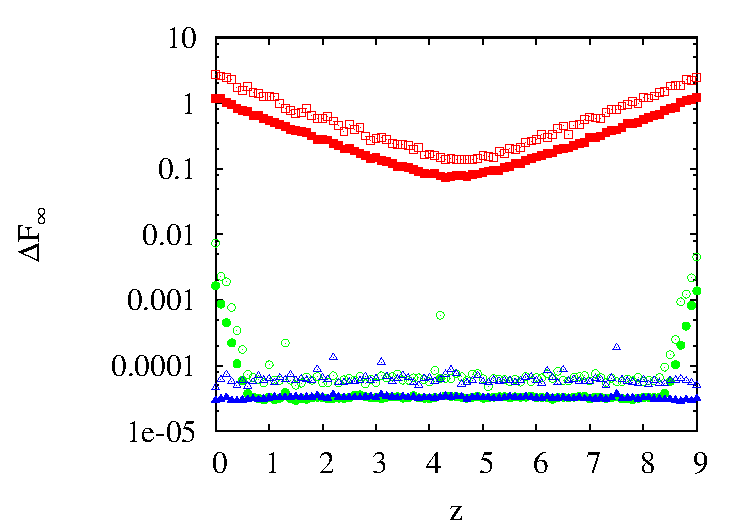
\includegraphics[width=0.4\textwidth]{figures/elc-errordist}
  \caption{Error distribution of the ELC method.}
  \label{fig:ELC-error}
\end{figure}

Figure \ref{fig:ELC-error} shows the error distribution of the ELC
method for a gap size of $10\%$ of the total system height. For MMM2D
and MMM1D the error distribution is less homogenous, however, also
here it is always better to have some extra precision, especially
since it is computationally cheap.


%%% Local Variables: 
%%% mode: latex
%%% TeX-master: "ug"
%%% End: 
